\subsection{Mục tiêu và đặc điểm dữ liệu}
\label{subsec:db_muc_tieu}

Cơ sở dữ liệu PostgreSQL của Yoca được thiết kế theo hai lớp có mục đích khác nhau. Lớp thứ nhất là dữ liệu nền tương đối chuẩn hóa, gồm tài khoản, phương thức xác thực, watchlist, nhãn ví, cảnh báo, subscription và thanh toán. Đây là dữ liệu do người dùng hoặc hệ thống sở hữu, cần khóa ngoại và quy tắc xóa rõ ràng. Lớp thứ hai là các read model và cache bền vững cho token, pool, ví, giao dịch và kết quả phân tích. Lớp này ưu tiên khả năng đọc nhanh, tái sử dụng dữ liệu provider và làm mới từng phần hơn là loại bỏ mọi sự lặp dữ liệu.

Dữ liệu trong Yoca có hai đặc điểm. Dữ liệu tài khoản và thanh toán cần quan hệ rõ ràng, ràng buộc khóa ngoại và quy tắc xóa nhất quán. Ngược lại, phần lớn dữ liệu blockchain là dữ liệu công khai được định danh bằng token address, wallet address hoặc transaction signature. Các bảng này thường không phụ thuộc vào một bảng gốc duy nhất mà được liên kết theo khóa nghiệp vụ.

Schema được định nghĩa bằng Drizzle ORM. Kiểu dữ liệu, primary key, unique constraint và foreign key được đặt trong mã TypeScript, giúp truy vấn backend và cấu trúc PostgreSQL dùng chung một định nghĩa. Tuy nhiên, schema vật lý không phải lúc nào cũng trùng với mô hình khái niệm: wallet address, token address và signature thường là khóa nghiệp vụ liên kết nhiều bảng nhưng không bị buộc phải tham chiếu đến một bảng cha.

\subsection{Phân nhóm dữ liệu theo miền nghiệp vụ}
\label{subsec:db_phan_nhom}

Cấu trúc lưu trữ được chia theo các miền identity/payment, token/market, wallet/analysis, transaction, alert và content/AI. Hình~\ref{fig:db_overview} chỉ thể hiện quan hệ khái niệm giữa các miền; các ERD phía sau mới phân biệt foreign key vật lý với liên hệ bằng address hoặc signature.

\begin{figure}[H]
    \centering
    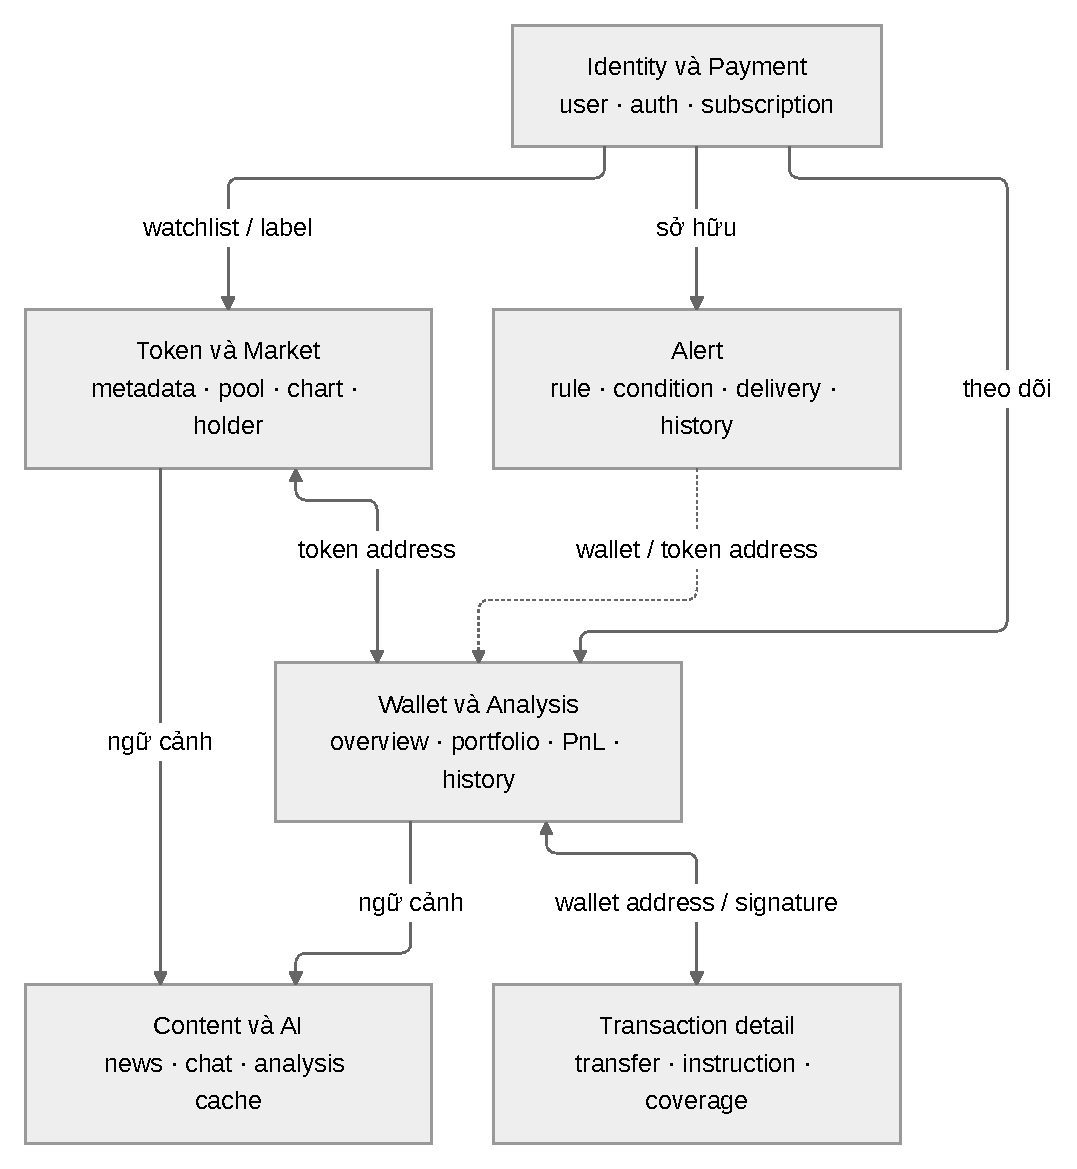
\includegraphics[width=0.9\textwidth,height=0.68\textheight,keepaspectratio]{Chapter3/diagrams/database-overview.pdf}
    \caption{Các miền dữ liệu chính và quan hệ khái niệm}
    \label{fig:db_overview}
\end{figure}

Các nhóm trên phục vụ nhu cầu truy vấn khác nhau. Vì vậy, dữ liệu có thể giao nhau về wallet address, token address hoặc transaction signature nhưng không đồng nghĩa các bảng có thể thay thế trực tiếp cho nhau. Cách phân nhóm cũng giúp ERD tổng thể không biến thành một hình quá dài theo chiều ngang và phải thu nhỏ đến mức không đọc được.
